\documentclass[xcolor={usenames,dvipsnames}]{beamer}

\usepackage[T1]{fontenc}
%\usepackage{totcount}
%\regtotcounter{section}
%\usepackage{multido}
\usepackage{verbatim}
\usepackage{listings}

\title{Introduction to Dependent Types}
\subtitle{Eagan Technology Unconference}
\author{Joseph Ching}
\date{September 11, 2015}

\usetheme{Antibes}
\usecolortheme{beaver}

% http://tex.stackexchange.com/questions/131515/show-hide-subsections-in-the-table-of-contents-of-a-beamer-presentation
%\newcommand{\mytableofcontents}[0]{
%  \multido{\I=1+1}{\totvalue{section}}{
%    \begin{frame}<beamer>
%      \setcounter{section}{\I}
%      \frametitle{Outline}
%      \tableofcontents[
%      currentsection,
%      sectionstyle=show/show,
%      subsectionstyle=show/show/hide,
%      ]
%    \end{frame}
%  }
%  \setcounter{section}{0}
%}
% http://tex.stackexchange.com/questions/108898/beamer-presentation-show-toc-at-beginning-of-unnumbered-subsection-subsection
%\AtBeginSection[
%{\frame<beamer>{\frametitle{Outline}
%    \tableofcontents[currentsection]}}
%]
%{\frame<beamer>{
%    \frametitle{Outline}
%    \tableofcontents[currentsection]}
%}
% https://www.sharelatex.com/learn/Beamer
\AtBeginSection[] {
  \begin{frame}
    \frametitle{Section Outline}
    \tableofcontents[
      currentsection,
      sectionstyle=show/hide,
      subsectionstyle=show/show/hide
    ]
  \end{frame}
}
\newcommand{\hkeyword}[1]{\textcolor{Aquamarine}{\textsc{#1}}}
\newcommand{\hfunction}[1]{\textcolor{OliveGreen}{\textsc{#1}}}
\newcommand{\htycon}[1]{\textcolor{MidnightBlue}{\textsc{#1}}}
\newcommand{\hvalcon}[1]{\textcolor{Red}{\textsc{#1}}}
\newcommand{\hkind}[1]{\textcolor{Fuchsia}{\textsc{#1}}}
\newcommand{\hsort}[1]{\textcolor{Orange}{\textsc{#1}}}
\newcommand{\hclass}[1]{\textcolor{Magenta}{\textsc{#1}}}
\newcommand{\htyfam}[1]{\textcolor{Green}{\textsc{#1}}}
\newcommand{\hcomment}[1]{\textcolor{Grey}{\textsc{#1}}}
\newcommand{\hother}[1]{\textcolor{Black}{\textsc{#1}}}

\lstdefinestyle{hask}{
  basicstyle=\ttfamily\scriptsize\color{Black},
  sensitive=true,
  morecomment=[l][\color{Gray}\ttfamily\tiny]{--},
  morecomment=[s][\color{Gray}\ttfamily\tiny]{\{-}{-\}},
  morestring=[b]",
  stringstyle=\color{Maroon},
  showstringspaces=false,
  numberstyle=\color{Red},
  numberblanklines=true,
  showspaces=false,
  breaklines=true,
  showtabs=false,
  moredelim=**[is][\color{Aquamarine}]{@kw}{@},
  moredelim=**[is][\color{OliveGreen}]{@f}{@},
  moredelim=**[is][\color{MidnightBlue}]{@tc}{@},
  moredelim=**[is][\color{Red}]{@vc}{@},
  moredelim=**[is][\color{Fuchsia}]{@dk}{@},
  moredelim=**[is][\color{Orange}]{@st}{@},
  moredelim=**[is][\color{Magenta}]{@cc}{@},
  moredelim=**[is][\color{Green}]{@tf}{@},
  moredelim=**[is][\color{Maroon}]{@str}{@},
  moredelim=**[is][\color{Black}]{@o}{@},
  escapeinside={{@|}{@}},
  % Keywords
  emph=
  {[1]
    % as didn't make it due to a:as
    module,import,qualified,hiding,foreign,infix,infixr,infixl,
    where,let,in,case,of,if,then,else,do,rec,proc,forall,pi,with,
    type,newtype,data,family,kind,class,instance,deriving,default
  },
  emphstyle={[1]\color{Aquamarine}\textbf},
  % functions
  emph=
  {[2]
    placeholder
  },
  emphstyle={[2]\color{OliveGreen}},
  % type constructors
  emph=
  {[3]
    Char,String,Bool,Int,Integer,Double,Float,Ordering,Maybe,Either,IO,
    List, Vect, Func, HList, HVect
  },
  emphstyle={[3]\color{MidnightBlue}\textbf},
  emph=
  % value constructors
  {[4]
    True,False,Nothing,Just,Left,Right,LT,EQ,GT,
    Nil, Cons, VNil, VCons, HNil, HCons, HVNil, HVCons
  },
  emphstyle={[4]\color{Red}\textbf},
  % type classes, contexts, constraints
  emph=
  {[5]
    Show,Read,Eq,Ord,Enum,Bounded,Num,
    Monoid,Functor,Foldable,Traversable,Applicative,Alternative,Monad,Comonad,Arrow
  },
  emphstyle={[5]\color{Magenta}\textbf},
  % kinds
  emph=
  {[6]
    Constraint,AnyK,OpenKind
  },
  emphstyle={[6]\color{Fuchsia}\textbf},
  % sort
  emph=
  {[8]
    BOX
  },
  emphstyle={[8]\color{Orange}\textbf},
  % type families
  emph=
  {[8]
    Sing,Plus,Mult,Min
  },
  emphstyle={[8]\color{Green}\textbf},
  % foreign languages
  emph=
  {[9]
    enum, interface, new, static, switch, return
  },
  emphstyle={[9]\color{Aquamarine}\textbf},
}

\begin{document}


%%%%%%%%%%%%%%%%%%%%%%%%%%%%%%%%%%%%%%%%%%%%%%%%%%%%%%%%%%%%%%%%%%%%%%%%%%%%%%%%
%%% Title Page
%%%%%%%%%%%%%%%%%%%%%%%%%%%%%%%%%%%%%%%%%%%%%%%%%%%%%%%%%%%%%%%%%%%%%%%%%%%%%%%%
\begin{frame}[plain]
  \titlepage
\end{frame}


%%%%%%%%%%%%%%%%%%%%%%%%%%%%%%%%%%%%%%%%%%%%%%%%%%%%%%%%%%%%%%%%%%%%%%%%%%%%%%%%
%%% Table of Content
%%%%%%%%%%%%%%%%%%%%%%%%%%%%%%%%%%%%%%%%%%%%%%%%%%%%%%%%%%%%%%%%%%%%%%%%%%%%%%%%
% Want to hide subsection slide by slide
\begin{frame}{Agenda}
  \tableofcontents[
%   pausesections,
    sectionstyle=show,
    subsectionstyle=hide
  ]
\end{frame}
%\mytableofcontents


%%%%%%%%%%%%%%%%%%%%%%%%%%%%%%%%%%%%%%%%%%%%%%%%%%%%%%%%%%%%%%%%%%%%%%%%%%%%%%%%
%%% Preface
%%%%%%%%%%%%%%%%%%%%%%%%%%%%%%%%%%%%%%%%%%%%%%%%%%%%%%%%%%%%%%%%%%%%%%%%%%%%%%%%
\section{Preface}

\begin{frame}{Quick Question}
  How many are familiar with this topic?
\end{frame}

\begin{frame}{A Joke}
  This is not a \texttt{m-} tutorial, and nothing here will involve burritos.
\end{frame}

\begin{frame}{Disclaimer}
  There will be many code examples with \textit{very} loose translations to imperative/OOP as we go along. Though please keep in mind that these are merely made up syntactical translations, the actual concepts may differ vastly.
\end{frame}

\begin{frame}{About This Talk}
  Example languages with dependent types:
  \begin{itemize}
    \item \texttt{Idris}
    \item \texttt{Epigram}
    \item \texttt{Agda}
    \item \texttt{Coq}
  \end{itemize}

    \ \\
    \pause
    But we will be using \texttt{Haskell} though.

    \ \\
    \ \\
    \textit{\tiny{Honestly, it's because they're way over his head...}}\\
\end{frame}

\begin{frame}[fragile]{Dependent Types}
  Why do we want them?
  \begin{itemize}
    \item more expressive \texttt{type system}
    \item encode stronger invariants
    \item proving correctness of code
  \end{itemize}
\end{frame}

\begin{frame}[fragile]{Teaser}
  Example please:
  \begin{lstlisting}[style=hask]
    infixr @vc5@ @vc:>@
    data Vect (n :: @dkNat@) a where
      VNil :: Vect @vc0@ a
      (@vc:>@) :: a -> Vect n a -> Vect (n @tf+@ @vc1@) a

    vs :: Vect @vc6@ Int
    vs = @vc4@ @vc:>@ @vc8@ @vc:>@ @vc15@ @vc:>@ @vc16@ @vc:>@ @vc23@ @vc:>@ @vc42@ @vc:>@ VNil
  \end{lstlisting}

  Translation\textsuperscript{*} please:
  \begin{lstlisting}[style=hask]
    enum Vect<@dkNat@ n, A> {
      Vect<@vc0@, A> VNil,
      Vect<n @tf'+@ @vc1@, A> VCons(A a, Vect<n, A> va)
    }

    Vect<@vc6@, Int> vs = VCons(@vc4@, VCons(@vc8@, VCons(@vc15@, VCons(@vc16@, VCons(@vc23@, VCons(@vc42@, VNil))))));
  \end{lstlisting}
  \textit{\tiny{(*) supreme looseness and totally made-up syntax!!!}}
\end{frame}


%%%%%%%%%%%%%%%%%%%%%%%%%%%%%%%%%%%%%%%%%%%%%%%%%%%%%%%%%%%%%%%%%%%%%%%%%%%%%%%%
%%% Introduction
%%%%%%%%%%%%%%%%%%%%%%%%%%%%%%%%%%%%%%%%%%%%%%%%%%%%%%%%%%%%%%%%%%%%%%%%%%%%%%%%
\section{Review of Basics}

%%%%%%%%%%%%%%%%%%%%%%%%%%%%%%%%%%%%%%%%%%%%%%%%%%%%%%%%%%%%%%%%%%%%%%%%%%%%%%%%
\subsection{Values and Types}

\begin{frame}[fragile]{Values and Types}
  \hvalcon{Values} has \htycon{Types}, or \hvalcon{Values} are classified by \htycon{Types}.\\

  \begin{lstlisting}[style=hask]
    @|\ldots@, @vc-1@, @vc0@, @vc1@, @vc2@, @vc3@, @|\dots@ :: Int

    True, False :: Bool

    @str'a'@, @str'b'@, @str'c'@ :: Char

    "abc" :: String @|$\sim$@ @tc[@Char@tc]@
  \end{lstlisting}
\end{frame}

\begin{frame}[fragile]{About Data Types}
  How are data types defined?\\
  \begin{itemize}
    \item Some are built in magic: \htycon{Int}, \htycon{Char}, function arrow
    \item Some are built in sugar: list, tuples
      \begin{itemize}
        \item We can define equivalent non-sugar version ourselves
      \end{itemize}
    \item Rest can be user defined: \htycon{Bool}, \htycon{String}, \htycon{Maybe}
  \end{itemize}
\end{frame}

\begin{frame}[fragile]{About Data Types}
  What are the data types like?
  \begin{itemize}
    \item Multiple \hvalcon{Value} constructors
    \item Paremetrize over another \htycon{Type}
    \item Recursive definition
    \item Synonyms of other \htycon{Types}
    \item Combination of the above
  \end{itemize}
\end{frame}

%%%%%%%%%%%%%%%%%%%%%%%%%%%%%%%%%%%%%%%%%%%%%%%%%%%%%%%%%%%%%%%%%%%%%%%%%%%%%%%%
\subsection{Defining Data Types}
\begin{frame}[fragile]{Defining Data Types}
  Define new data type with \hkeyword{data}.

  \ \\
  \begin{itemize}
    \item Left hand side (LHS) - \htycon{Type} constructor
    \item Right hand side (RHS) - \hvalcon{Value} constructor
  \end{itemize}

  \ \\
  \htycon{Type} and \hvalcon{Value} constructors are capticalized.
\end{frame}

\begin{frame}[fragile]{Our First Example!}
  Define a person:
  \begin{lstlisting}[style=hask]
    -- | params for firstname, lastname, age respectively
    data @tcPerson@ = @vcPerson@ String String Int

    barbara :: @tcPerson@
    barbara = @vcPerson@ "Barbara" "Smith" @vc30@
  \end{lstlisting}

  The \htycon{Type} of the \hvalcon{Person Value} constructor:
  \begin{lstlisting}[style=hask]
    @vcPerson@ :: String -> String -> Int -> @tcPerson@
  \end{lstlisting}

  A loose translation:
  \begin{lstlisting}[style=hask]
    enum @tcPerson@ {
      @vcPerson@(String firstname, String lastname, Int age)
    }

    @tcPerson@ barbara = new @vcPerson@("Barbara", "Smith", @vc30@)
  \end{lstlisting}
\end{frame}

\begin{frame}[fragile]{Multiple Value Constructors}
  Data can have multiple \hvalcon{Value} constructors:
  \begin{lstlisting}[style=hask]
    data Bool = False | True

    data @tcWeekdays@ = @vcSunday@ | @vcMonday@ | @vcTuesday@ | @vcWednesday@
                  | @vcThursday@ | @vcFriday@ | @vcSaturday@
  \end{lstlisting}
% \textit{\tiny{Does this remind you of anything?}}

  A loose translation:
  \begin{lstlisting}[style=hask]
    enum Bool { False, True }

    enum @tcWeekdays@ {
      @vcSunday@, @vcMonday@, @vcTuesday@, @vcWednesday@, @vcThursday@, @vcFriday@, @vcSaturday@
    }
  \end{lstlisting}
\end{frame}

\begin{frame}[fragile]{Multiple Value Constructor}
  You can do type aliasing with \hkeyword{type}:
  \begin{lstlisting}[style=hask]
    type String = @tc[@Char@tc]@
    type @tcSide@ = Double
    type @tcRadius@ = Double
  \end{lstlisting}

  For example:
  \begin{lstlisting}[style=hask]
    data @tcShape@ = @vcTriangle@ @tcSide@ @tcSide@ @tcSide@
               | @vcRectangle@ @tcSide@ @tcSide@
               | @vcCircle@ @tcRadius@
  \end{lstlisting}

  A loose translation:
  \begin{lstlisting}[style=hask]
    enum @tcShape@ {
      @vcTriangle@(Double side1, Double side2, Double side3),
      @vcRectangle@(Double length, Double width),
      @vcCircle@(Double radius)
    }
  \end{lstlisting}
\end{frame}

\begin{frame}[fragile]{Multiple Value Constructor}
  Recall \htycon{Side} $\sim$ \htycon{Radius} $\sim$ \htycon{Double}:
  \begin{lstlisting}[style=hask]
    data @tcShape@ = @vcTriangle@ @tcSide@ @tcSide@ @tcSide@
               | @vcRectangle@ @tcSide@ @tcSide@
               | @vcCircle@ @tcRadius@
  \end{lstlisting}

  \htycon{Types} of the 3 \hvalcon{Value} constructors:
  \begin{lstlisting}[style=hask]
    @vcTriangle@  :: @tcSide@ -> @tcSide@ -> @tcSide@ -> @tcShape@
    @vcRectangle@ :: @tcSide@ -> @tcSide@ -> @tcShape@
    @vcCircle@    :: @tcRadius@ -> @tcShape@
  \end{lstlisting}

  Example \htycon{Shapes}:
  \begin{lstlisting}[style=hask]
    myTri, myRect, myCir :: @tcShape@
    myTri  = @vcTriangle@ @vc2.1 3.2 5@
    myRect = @vcRectangle@ @vc4 4@
    myCir  = @vcCircle@ @vc7.2@
  \end{lstlisting}
\end{frame}

\begin{frame}[fragile]{Parametrization}
  Types can parametrize over another type:
  \begin{lstlisting}[style=hask]
    data @tcTuple@ a b = @vcTuple@ a b
  \end{lstlisting}

  With:
  \begin{lstlisting}[style=hask]
    @vcTuple@ :: a -> b -> @tcTuple@ a b
  \end{lstlisting}

  A loose translation:
  \begin{lstlisting}[style=hask]
    enum @tcTuple@<A, B> {
      @vcTuple@(A a, B b)
    }
  \end{lstlisting}
\end{frame}

\begin{frame}[fragile]{Tuple}
  Actual built-in sugar:
  \begin{lstlisting}[style=hask]
       data @tcTuple@ a b = @vcTuple@ a b
    => data (@tc,@) a b = (@vc,@) a b
    => data (a@tc,@ b) = (a@vc,@ b)
  \end{lstlisting}

  An example:
  \begin{lstlisting}[style=hask]
    type @tcEmployed@ = Bool

    barbara, chet, luffy :: (@tcPerson@@tc,@ @tcEmployed@)
    barbara = (@vcPerson@ "Barbara" "Smith" @vc30,@ True)
    chet    = (@vcPerson@ "Chet" "Awesome-Laser" @vc2,@ False)
    luffy   = (@vcPerson@ "Luffy D." "Monkey" @vc19,@ False)
  \end{lstlisting}
\end{frame}

\begin{frame}[fragile]{Maybe}
  Like \htycon{Bool}, but parametrizes a \htycon{Type} $a$ over the \htycon{True} part:
  \begin{lstlisting}[style=hask]
    data Maybe a = Nothing | Just a
  \end{lstlisting}

  With:
  \begin{lstlisting}[style=hask]
    Nothing :: Maybe a
    Just    :: a -> Maybe a
  \end{lstlisting}

  A loose translation:
  \begin{lstlisting}[style=hask]
    enum Maybe<A> {
      Nothing,
      Just(A a)
    }
  \end{lstlisting}
\end{frame}

\begin{frame}[fragile]{Maybe}
  From previous slide:
  \begin{lstlisting}[style=hask]
    data Maybe a = Nothing | Just a
  \end{lstlisting}

  Say more with \htycon{Occupation}:
  \begin{lstlisting}[style=hask]
    type @tcOccupation@ = Maybe String

    barbara2, chet2, luffy2 :: (@tcPerson@@tc,@ @tcOccupation@)
    barbara2 = (@vcPerson@ "Barbara" "Smith" @vc30,@ Just "dancer")
    chet2    = (@vcPerson@ "Chet" "Awesome-Laser" @vc2,@ Nothing)
    luffy2   = (@vcPerson@ "Luffy D." "Monkey" @vc19,@ Just "pirate")
  \end{lstlisting}
\end{frame}

\begin{frame}[fragile]{Types with Recursion}
  Natural number:
  \begin{lstlisting}[style=hask]
    data @tcNat@ = @vcZ@ | @vcS@ @tcNat@
  \end{lstlisting}

  With:
  \begin{lstlisting}[style=hask]
    @vcZ@ :: @tcNat@
    @vcS@ :: @tcNat@ -> @tcNat@
  \end{lstlisting}

  A loose translation:
  \begin{lstlisting}[style=hask]
    enum @tcNat@ {
      @vcZ@,
      @vcS@(@tcNat@ n)
    }
  \end{lstlisting}
\end{frame}

\begin{frame}[fragile]{Types with Recursion}
  Natural number:
  \begin{lstlisting}[style=hask]
    data @tcNat@ = @vcZ@ | @vcS@ @tcNat@

    @vcZ@ :: @tcNat@
    @vcS@ :: @tcNat@ -> @tcNat@

    @vc0@ @|$\sim$@ @vcZ@
    @vc1@ @|$\sim$@ @vcS@ @vcZ@
    @vc2@ @|$\sim$@ @vcS@ (@vcS@ @vcZ@)
    @vc3@ @|$\sim$@ @vcS@ (@vcS@ (@vcS@ @vcZ@))
  \end{lstlisting}
\end{frame}

\begin{frame}[fragile]{Types with Recursion}
  \htycon{List} - recursive \htycon{Type} that parametrizes over another \htycon{Type}:
  \begin{lstlisting}[style=hask]
    data List a = Nil | Cons a (List a)
  \end{lstlisting}

  With:
  \begin{lstlisting}[style=hask]
    Nil  :: List a
    Cons :: a -> List a -> List a
  \end{lstlisting}

  A loose translation:
  \begin{lstlisting}[style=hask]
    enum List<A> {
      Nil,
      Cons(A a, List<A> as)
    }
  \end{lstlisting}
\end{frame}

\begin{frame}[fragile]{Types with Recursion}
  Actual built-in sugar is something like:
  \begin{lstlisting}[style=hask]
       data List a = Nil | Cons a (List a)
    => data @tc[]@ a = @vc[]@ | (@vc:@) a (@tc[]@ a)
    => data @tc[@a@tc]@ = @vc[]@ | (@vc:@) a @tc[@a@tc]@
  \end{lstlisting}

  Sugar that \htycon{List}:
  \begin{lstlisting}[style=hask]
    ints :: List Int 
    ints = Cons 1 (Cons 2 (Cons 3 (Cons 4 Nil)))

    -- built-in sugar
    ints :: @tc[]@ Int
    ints = 1 @vc:@ 2 @vc:@ 3 @vc:@ 4 @vc:@ @vc[]@

    -- 2x the sugar!
    ints :: @tc[@Int@tc]@
    ints = @vc[@1, 2, 3, 4@vc]@
  \end{lstlisting}
\end{frame}


%%%%%%%%%%%%%%%%%%%%%%%%%%%%%%%%%%%%%%%%%%%%%%%%%%%%%%%%%%%%%%%%%%%%%%%%%%%%%%%%
\subsection{Functions}

\begin{frame}[fragile]{Functions}
  Maps \hvalcon{Values} of a \htycon{Type} to \hvalcon{Values} of another \htycon{Type}:
  \begin{lstlisting}[style=hask]
    even :: Int -> Bool
    even @vc0@ = True
    even n = if rem n @vc2@ == @vc0@
             then True
             else False
  \end{lstlisting}

  Not as loose translation:
  \begin{lstlisting}[style=hask]
    Bool even(Int n) {
      switch n:
        case n == @vc0@:
          return True;
        default:
          if rem(n, @vc2@) == @vc0@
            return True;
          else
            return False;
    }
  \end{lstlisting}
\end{frame}

\begin{frame}[fragile]{Functions with Recursion}
  Use recursion for recursive \htycon{Types}:
  \begin{lstlisting}[style=hask]
    data @tcNat@ = @vcZ@ | @vcS@ @tcNat@

    toInt :: @tcNat@ -> Int
    toInt @vcZ@     = @vc0@
    toInt (@vcS@ n) = @vc1@ + toInt n
  \end{lstlisting}

  Not as loose translation:
  \begin{lstlisting}[style=hask]
    Int toInt(@tcNat@ n) {
      switch n:
        case @vcZ@:
          return @vc0@;
        case (@vcS@ m):  -- n @|$\sim$@ (S m)
          return @vc1@ + toInt(m);
    }
  \end{lstlisting}
\end{frame}

\begin{frame}[fragile]{Functions with Recursion}
  Use recursion for recursive \htycon{Types}:
  \begin{lstlisting}[style=hask]
    data @tcNat@ = @vcZ@ | @vcS@ @tcNat@

    toInt :: @tcNat@ -> Int
    toInt @vcZ@     = @vc0@
    toInt (@vcS@ n) = @vc1@ + toInt n
  \end{lstlisting}

  Evaluation is a series of substitutions:
  \begin{lstlisting}[style=hask]
    three = @vcS@ (@vcS@ (@vcS@ @vcZ@)) :: @tcNat@

      toInt three :: Int
    = toInt (@vcS@ (@vcS@ (@vcS@ @vcZ@)))
    = @vc1@ + toInt (@vcS@ (@vcS@ @vcZ@))
    = @vc1@ + @vc1@ + toInt (@vcS@ @vcZ@)
    = @vc1@ + @vc1@ + @vc1@ + toInt @vcZ@
    = @vc1@ + @vc1@ + @vc1@ + @vc0@
    = @vc1@ + @vc1@ + @vc1@
    = @vc1@ + @vc2@
    = @vc3@
  \end{lstlisting}
\end{frame}

\begin{frame}[fragile]{Functions with Parametric Polymorphism}
  Functions can be parametric:
  \begin{lstlisting}[style=hask]
    data @tc[@a@tc]@ = @vc[]@ | (@vc:@) a @tc[@a@tc]@

    length :: @tc[@a@tc]@ -> Int
    length @vc[]@     = @vc0@
    length (x@vc:@xs) = @vc1@ + length xs
  \end{lstlisting}

  A translation:
  \begin{lstlisting}[style=hask]
    Int length(List<A> ls) {
      switch ls:
        case Nil:
          return @vc0@;
        case Cons(x, xs):
          return @vc1@ + length(xs);
    }
  \end{lstlisting}
\end{frame}

\begin{frame}[fragile]{Functions with Parametric Polymorphism}
  Functions can be parametric:
  \begin{lstlisting}[style=hask]
    data @tc[@a@tc]@ = @vc[]@ | (@vc:@) a @tc[@a@tc]@

    length :: @tc[@a@tc]@ -> Int
    length @vc[]@     = @vc0@
    length (x@vc:@xs) = 1 + length xs
  \end{lstlisting}

  Evaluation is a series of substitutions:
  \begin{lstlisting}[style=hask]
    xs = @vc[@@vc4@, @vc8@@vc@, @vc15@@vc]@ = @vc4@ @vc:@ @vc8@ @vc:@ @vc15@ @vc:@ @vc[]@ :: @tc[@Int@tc]@

      length xs :: Int
    = length @vc[@@vc4@, @vc8@, @vc15@@vc]@
    = @vc1@ + length @vc[@@vc8@, @vc15@@vc]@
    = @vc1@ + @vc1@ + length @vc[@@vc15@@vc]@
    = @vc1@ + @vc1@ + @vc1@ + length @vc[]@
    = @vc1@ + @vc1@ + @vc1@ + @vc0@
    = @vc1@ + @vc1@ + @vc1@
    = @vc1@ + @vc2@
    = @vc3@
  \end{lstlisting}
\end{frame}

\begin{frame}[fragile]{Higher-order Functions}
  Functions that take functions as params:
  \begin{lstlisting}[style=hask]
    -- actual name is ($)
    apply :: (a -> b) -> a -> b
    apply f x = f x

    -- acutal name is (.)
    compose :: (b -> c) -> (a -> b) -> (a -> c)
    compose f g = \x -> f (g x)
  \end{lstlisting}

  Yay translations:
  \begin{lstlisting}[style=hask]
    B apply(Func<A, B> f, A a) {
      return f(a);
    }

    Func<A, C> compose(Func<B, C> f, Func<A, B> g) {
      return x => f(g(x));
    }
  \end{lstlisting}
\end{frame}


%%%%%%%%%%%%%%%%%%%%%%%%%%%%%%%%%%%%%%%%%%%%%%%%%%%%%%%%%%%%%%%%%%%%%%%%%%%%%%%%
%%% Type Theory
%%%%%%%%%%%%%%%%%%%%%%%%%%%%%%%%%%%%%%%%%%%%%%%%%%%%%%%%%%%%%%%%%%%%%%%%%%%%%%%%
\section{What is Dependent Type}

%%%%%%%%%%%%%%%%%%%%%%%%%%%%%%%%%%%%%%%%%%%%%%%%%%%%%%%%%%%%%%%%%%%%%%%%%%%%%%%%
\subsection{$\lambda$-Calculus}

\begin{frame}[fragile]{$\lambda$-Calculus}
  So far, we have seen:
  \begin{itemize}
    \item function application
    \item function abstraction {\tiny(aka higher-order functions)}
    \item variable binding
    \item substitution
  \end{itemize}
  => basis for \texttt{simply typed $\lambda$-calculus}.
\end{frame}

\begin{frame}[fragile]{$\lambda$-Calculus}
  You: Sure...\\
  Me: Ah, yes, we want to extend \texttt{$\lambda$-calculus} so we can have more forms of abstractions!

  \ \\
  \pause
  Q: But how?\\
  A: What if I tell you\ldots\\
  \qquad \ldots you should already be familiar with 2 axes of extension :)
\end{frame}


%%%%%%%%%%%%%%%%%%%%%%%%%%%%%%%%%%%%%%%%%%%%%%%%%%%%%%%%%%%%%%%%%%%%%%%%%%%%%%%%
\subsection{Extensions on $\lambda$-calculus}

\begin{frame}[fragile]{Subtype Polymorphism}
  Given data types \htycon{$T$} and \htycon{$P$}, if there is a relation between \htycon{$T$} and \htycon{$P$} by some notion of substitutability with \htycon{$T$} in place of \htycon{$P$}, then we say \htycon{$T$} is a \texttt{subtype} of the \texttt{supertype} \htycon{$P$}, denoted by \htycon{$T$} $<:$ \htycon{$P$}.

  \ \\
  The is an extension on \texttt{$\lambda$-calculus} with \texttt{subtype polymorphism} and is denoted by $\lambda_{<:}$.\\
  => \texttt{Object Oriented Programming}
  
  \ \\
  \scriptsize{Though this is not an axis that we are interested in}.
\end{frame}

\begin{frame}[fragile]{Parametric Polymorphism}
  Introduce a mechanism of \texttt{universal quantification} over \htycon{Types}: \htycon{Types} can abstract over \htycon{Types}, allows for \texttt{generic data types} and \texttt{generic functions}.\\
  => \texttt{Generic Programming}

  \ \\
  Recall:
  \begin{lstlisting}[style=hask]
    data Maybe a = Nothing | Just a
    data List a = Nil | Cons a (List a)

    (.) :: (b -> c) -> (a -> b) -> (a -> c)
    map :: (a -> b) -> @tc[@a@tc]@ -> @tc[@b@tc]@
  \end{lstlisting}

  The name for this extension is formally \texttt{second order $\lambda$-calculus}, aka \texttt{System F}, denoted by $\lambda2$,
\end{frame}

\begin{frame}[fragile]{Value and Type Interdependency}
  Re-thinking functions:
  \begin{lstlisting}[style=hask]
    even :: Int -> Bool
    even @vc0@ = True
    even n = if rem n @vc2@ == @vc0@
             then True
             else False
  \end{lstlisting}

  \qquad \texttt{even} maps \hvalcon{Int}s to \hvalcon{True} and \hvalcon{False}.
  \ \\
  => \hvalcon{Values} on RHS depends on the \hvalcon{Values} on LHS
  \ \\
  => \hvalcon{Values} depending on \hvalcon{Values}
  \ \\
  => Ordinary \texttt{$\lambda$-calculus}
\end{frame}

\begin{frame}[fragile]{Value and Type Interdependency}
  Re-thinking parametrized data types:
  \begin{lstlisting}[style=hask]
    data Maybe a = Nothing | Just a

    data List a = Nil | Cons a (List a)
  \end{lstlisting}

  \qquad \htycon{Maybe} and \htycon{List} take a \htycon{Type} and return \hvalcon{Value} constructors
  \ \\
  => \hvalcon{Values} on RHS depends on the \htycon{Type} on LHS
  \ \\
  => \hvalcon{Values} depending on \htycon{Types}
  \ \\
  => \texttt{Parametric polymorphism} of $\lambda2$

%  \ \\
%  \textit{\tiny{Are we seeing a pattern yet?}}
\end{frame}

\begin{frame}[fragile]{Value and Type Interdependency}
  Then what about the other cases of dependencies?
  \begin{itemize}
    \item \hvalcon{Values} depending on \hvalcon{Values}: \texttt{$\lambda$-calculus}
    \item \hvalcon{Values} depending on \htycon{Types}: $\lambda2$, \texttt{System F}
    \pause
    \item \htycon{Types} depending on \htycon{Types}: $\lambda\underline\omega$\\
      => \texttt{Type-level programming} via \texttt{type operators}
    \pause
    \item \htycon{Types} depending on \hvalcon{Values}: $\lambda\Pi$\\
      => \texttt{Dependent types}
  \end{itemize}
\end{frame}

\begin{frame}[fragile]{Lambda Cube}
  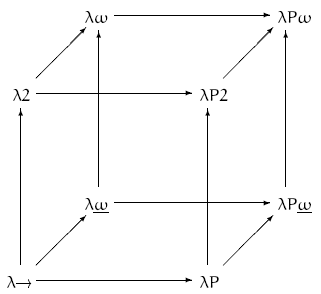
\includegraphics[scale=0.6]{Lambda_cube.png}
\end{frame}

\begin{frame}[fragile]{System F$_c$}
  Currently, \texttt{Haskell} as of GHC 7.10.2
  \begin{itemize}
    \item no true \texttt{type operators}
    \item \texttt{type-level programming} through:
      \begin{itemize}
        \item \texttt{type families}
        \item \texttt{equalities} and \texttt{coercions} on \htycon{Types}
      \end{itemize}
  \end{itemize}

  \ \\
  This axis of extension on $\lambda2$ is termed \texttt{System F$_c$}.
\end{frame}

\begin{frame}[fragile]{System F$_c$}
  Currently, \texttt{Haskell} as of GHC 7.10.2
  \begin{itemize}
    \item not fully dependent either:
      \begin{itemize}
        \item strong distinction between \hvalcon{Values} and \htycon{Types}
      \end{itemize}
    \item emulate \texttt{dependent types} with:
      \begin{itemize}
        \item handful of \texttt{language extensions}
        \item \hkind{Kind} system
      \end{itemize}
  \end{itemize}
\end{frame}


%%%%%%%%%%%%%%%%%%%%%%%%%%%%%%%%%%%%%%%%%%%%%%%%%%%%%%%%%%%%%%%%%%%%%%%%%%%%%%%%
%%% Dependent type programming in Haskell
%%%%%%%%%%%%%%%%%%%%%%%%%%%%%%%%%%%%%%%%%%%%%%%%%%%%%%%%%%%%%%%%%%%%%%%%%%%%%%%%
\section{Steps toward Dependent Types}

%%%%%%%%%%%%%%%%%%%%%%%%%%%%%%%%%%%%%%%%%%%%%%%%%%%%%%%%%%%%%%%%%%%%%%%%%%%%%%%%
\subsection{Kinds}

\begin{frame}[fragile]{Kinds}
  Q: \htycon{Types} classify \hvalcon{Values}, but what classifies \htycon{Types}?\\
  A: \hkind{Kinds}
\end{frame}

\begin{frame}[fragile]{Introducing $\star$}
  \begin{lstlisting}[style=hask]
    -- built-in magic: infinitely many value constructors
    data Int = @|\ldots@ | @vc-1@ | @vc0@ | @vc1@ | @vc2@ | @|\ldots@
    data Bool = False | True
    data @tc[@a@tc]@ = Nil | (@vc:@) a @vc[@a@vc]@
    data Maybe a = Nothing | Just a
    data (a@tc,@ b) = (a@vc,@ b)

    Int :: @dk*@
    Bool :: @dk*@
    @tc[@Int@tc]@ :: @dk*@
    @tc[]@ :: @dk*@ -> @dk*@
    Maybe @tcPerson@ :: @dk*@
    Maybe :: @dk*@ -> @dk*@
    (@tcPerson@@tc,@ Bool) :: @dk*@
    (@tc,@) :: @dk*@ -> @dk*@ -> @dk*@
  \end{lstlisting}
\end{frame}

\begin{frame}[fragile]{Other Kinds}
  There are other \hkind{Kinds} aside from \hkind{*}:
  \begin{lstlisting}[style=hask]
    (@dk*@)         -- kind of fully realized type
    (@dk#@)         -- kind of unboxed stuff used internally
    Constraint  -- kind of constraints and type equality
    OpenKind    -- superkind of (*) and (#)
    AnyK        -- polymorphic kind for flexible arity
    @|\pause@
    -- the only sort, sorts classify kinds
    (@dk*@), (@dk#@), Constraint, OpenKind, AnyK :: @stBOX@
    @stBOX@ :: @stBOX@
  \end{lstlisting}

  All these \hkind{Kinds} are built-in and inferred as of GHC 7.10.2.
  
  \ \\
  \textit{\tiny{All of this will be changed with the next GHC 8.0.1 release.}}
\end{frame}


%%%%%%%%%%%%%%%%%%%%%%%%%%%%%%%%%%%%%%%%%%%%%%%%%%%%%%%%%%%%%%%%%%%%%%%%%%%%%%%%
\subsection{Language Extensions}

\begin{frame}[fragile]{Language Extensions}
  Compiler extensions that enable a variety of new functionalities:
  \begin{itemize}
    \item Syntax extension
    \item Type-level programming
    \item Generic deriving
    \item FFI
    \item Type disambiguation
    \item Typeclass extension
  \end{itemize}

  \ \\
  Each extension has a name, and is enabled with the LANGUAGE pragma.
\end{frame}

\begin{frame}[fragile]{GADTs}
  Define data and explicit give type signatures to the \hvalcon{Value} constructors.
  \begin{lstlisting}[style=hask]
    data Bool = False | True
    data Maybe a = Nothing | Just a
    data List a = Nil | Cons a (List a)
  \end{lstlisting}

  Becomes:
  \begin{lstlisting}[style=hask]
    {-# LANGUAGE GADTs #-}
    data Bool where
      False :: Bool
      True  :: Bool

    data Maybe a where
      Nothing :: Maybe a
      Just    :: a -> Maybe a

    data List a where
      Nil  :: List a
      Cons :: a -> List a -> List a
  \end{lstlisting}
\end{frame}

\begin{frame}[fragile]{GADTs}
  Define data and explicit give type signatures to the \hvalcon{Value} constructors.
  \begin{lstlisting}[style=hask]
    data Bool = False | True
    data Maybe a = Nothing | Just a
    data List a = Nil | Cons a (List a)
  \end{lstlisting}

  Loose translations:
  \begin{lstlisting}[style=hask]
    enum Bool {
      Bool False,
      Bool True
    }

    enum Maybe<A> {
      Maybe<A> Nothing,
      Maybe<A> Just(A a)
    }

    enum List<A> {
      List<A> Nil,
      List<A> Cons(A a, List<A> as)
    }
  \end{lstlisting}
\end{frame}

\begin{frame}[fragile]{KindSignatures}
  Specify the \hkind{Kind} of the \htycon{Type} variables:
  \begin{lstlisting}[style=hask]
    {-# LANGUAGE GADTs #-}
    {-# LANGUAGE KindSignatures #-}
    data Bool :: @dk*@ where
      False :: Bool
      True  :: Bool

    data Maybe :: @dk*@ -> @dk*@ where
      Nothing :: Maybe a
      Just    :: a -> Maybe a

    data List :: @dk*@ -> @dk*@ where
      Nil  :: List a
      Cons :: a -> List a -> List a
  \end{lstlisting}
\end{frame}

\begin{frame}[fragile]{DataKinds}
  \hkind{Kinds} are built-in; no user defined \hkind{Kinds}.

  \ \\
  Want \hvalcon{Values} at the \htycon{Type} level though!

  \ \\
  => \texttt{Data kind promotion} :)
\end{frame}

\begin{frame}[fragile]{DataKinds}
  Example:
  \begin{lstlisting}[style=hask]
    data Bool = False | True
  \end{lstlisting}

  With DataKinds, we get something like:
  \begin{lstlisting}[style=hask]
    {-# LANGUAGE DataKinds #-}
  \end{lstlisting}
  \begin{tabular}{l || c | c}
    \hkind{Kind} & \ & \hkind{Bool} \\
    \hline \htycon{Type} & \htycon{Bool} & \htycon{'}\hvalcon{True} | \htycon{'}\hvalcon{False} \\
    \hline \hvalcon{Value} & \hvalcon{True} | \hvalcon{False} & \ \\
  \end{tabular}
\end{frame}

\begin{frame}[fragile]{DataKinds}
  Example:
  \begin{lstlisting}[style=hask]
    data @tcNat@ = @vcZ@ | @vcS@ @tcNat@
  \end{lstlisting}

  With DataKinds, we get something like:
  \begin{lstlisting}[style=hask]
    {-# LANGUAGE DataKinds #-}
  \end{lstlisting}
  \begin{tabular}{l || c | c}
    \hkind{Kind} & \ & \hkind{Nat} \\
    \hline \htycon{Type} & \htycon{Nat} & \htycon{'}\hvalcon{Z} | \htycon{'}\hvalcon{S} \hkind{Nat} \\
    \hline \hvalcon{Value} & \hvalcon{Z} | \hvalcon{S} \htycon{Nat} & \ \\
  \end{tabular}
\end{frame}

\begin{frame}[fragile]{Type Families}
  \texttt{Type families} - type level functions, computed and checked at compile time.

  \ \\
  Comes in 2 flavors:
  \begin{itemize}
    \item type synonym families
    \item data families
  \end{itemize}

  \ \\
  and have a few options:
  \begin{itemize}
    \item associated vs. standalone
    \item open vs. closed\textsuperscript{1}
    \item injectivity\textsuperscript{2}
  \end{itemize}
\end{frame}

\begin{frame}[fragile]{Type Families}
  At \hvalcon{Value} level:
  \begin{lstlisting}[style=hask]
    data @tcNat@ = @vcZ@ | @vcS@ @tcNat@

    add :: @tcNat@ -> @tcNat@ -> @tcNat@
    add @vcZ@     m = m
    add (@vcS@ n) m = @vcS@ (add n m)

       add (@vcS@ (@vcS@ @vcZ@)) (@vcS@ @vcZ@)
    => @vcS@ (add (@vcS@ @vcZ@) (@vcS@ @vcZ@))
    => @vcS@ (@vcS@ (add @vcZ@ (@vcS@ @vcZ@)))
    => @vcS@ (@vcS@ (@vcS@ @vcZ@))
  \end{lstlisting}
\end{frame}

\begin{frame}[fragile]{Type Families}
  At \htycon{Type} level:
  \begin{lstlisting}[style=hask]
    {-# LANGUAGE DataKinds #-}
    {-# LANGUAGE TypeFamilies #-}

    data @tcNat@ = @vcZ@ | @vcS@ @tcNat@

    type family @tfAdd@ (n :: @dkNat@) (m :: @dkNat@) :: @dkNat@ where
      @tfAdd@ @tc'@@vcZ@     m = m
      @tfAdd@ (@tc'@@vcS@ n) m = @tc'@@vcS@ (@tfAdd@ n m)

       @tfAdd@ (@tc'@@vcS@ (@tc'@@vcS@ @tc'@@vcZ@)) (@tc'@@vcS@ @tc'@@vcZ@)
    => @tc'@@vcS@ (@tfAdd@ (@tc'@@vcS@ @tc'@@vcZ@) (@tc'@@vcS@ @tc'@@vcZ@))
    => @tc'@@vcS@ (@tc'@@vcS@ (@tfAdd@ @tc'@@vcZ@ (@tc'@@vcS@ @tc'@@vcZ@)))
    => @tc'@@vcS@ (@tc'@@vcS@ (@tc'@@vcS@ @tc'@@vcZ@))
  \end{lstlisting}
\end{frame}

\begin{frame}[fragile]{Type Operators}
  Allows usage of symbols in place of \htycon{Type} constructors and \htycon{Type} families.

  \begin{lstlisting}[style=hask]
    {-# LANGUAGE DataKinds #-}
    {-# LANGUAGE TypeFamilies #-}
    {-# LANGUAGE TypeOperators #-}

    data @tcNat@ = @vcZ@ | @vcS@ @tcNat@

    type family (@tf'+@) n m where
      @tc'@@vcZ@     @tf'+@ m = m
      (@tc'@@vcS@ n) @tf'+@ m = @tc'@@vcS@ (n @tf'+@ m)

       (@tc'@@vcS@ (@tc'@@vcS@ @tc'@@vcZ@)) @tf'+@ (@tc'@@vcS@ @tc'@@vcZ@)
    => @tc'@@vcS@ ((@tc'@@vcS@ @tc'@@vcZ@) @tf'+@ (@tc'@@vcS@ @tc'@@vcZ@))
    => @tc'@@vcS@ (@tc'@@vcS@ (@tc'@@vcZ@ @tf'+@ (@tc'@@vcS@ @tc'@@vcZ@)))
    => @tc'@@vcS@ (@tc'@@vcS@ (@tc'@@vcS@ @tc'@@vcZ@))
  \end{lstlisting}
\end{frame}


%%%%%%%%%%%%%%%%%%%%%%%%%%%%%%%%%%%%%%%%%%%%%%%%%%%%%%%%%%%%%%%%%%%%%%%%%%%%%%%%
\subsection{Dependent Type Programming with Vectors}

\begin{frame}[fragile]{Vectors}
  Like \htycon{List}, but also \textit{indexed} by \hkind{Nat} to indicate length.

  \ \\
  \htycon{List}:
  \begin{lstlisting}[style=hask]
    data List a where
      Nil  :: List a
      Cons :: a -> List a -> List a
  \end{lstlisting}

  \htycon{Vector}:
  \begin{lstlisting}[style=hask]
    -- 'Z @|$\sim$@ 0
    -- 'S n @|$\sim$@ n '+ 1
    data Vect (n :: @dkNat@) a where
      VNil :: Vect @vcZ@ a
      (@vc:>@) :: a -> Vect n a -> Vect (@vcS@ n) a

    type @tcSix@ = @vcS@ (@vcS@ (@vcS@ (@vcS@ (@vcS@ (@vcS@ @vcZ@)))))
    vs :: Vect @tcSix@ Int
    vs = @vc4@ @vc:>@ @vc8@ @vc:>@ @vc15@ @vc:>@ @vc16@ @vc:>@ @vc23@ @vc:>@ @vc42@ @vc:>@ VNil
  \end{lstlisting}
\end{frame}

\begin{frame}[fragile]{Vectors}
  Like \htycon{List}, but also indexed by \hkind{Nat} to indicate length.

  \htycon{List}:
  \begin{lstlisting}[style=hask]
    data List a where
      Nil  :: List a
      Cons :: a -> List a -> List a
  \end{lstlisting}

  Module GHC.TypeLits provide \texttt{type-level literals}:
  \begin{lstlisting}[style=hask]
    -- 'Z @|$\sim$@ 0
    -- 'S n @|$\sim$@ n '+ 1
    data Vect (n :: @dkNat@) a where
      VNil :: Vect @vc0@ a
      (@vc:>@) :: a -> Vect n a -> Vect (n @tf'+@ @vc1@) a

    vs :: Vect @vc6@ Int
    vs = @vc4@ @vc:>@ @vc8@ @vc:>@ @vc15@ @vc:>@ @vc16@ @vc:>@ @vc23@ @vc:>@ @vc42@ @vc:>@ VNil
  \end{lstlisting}
\end{frame}

\begin{frame}[fragile]{Head}
  \texttt{head} returns the first element of the \htycon{List}:
  \begin{lstlisting}[style=hask]
    -- from standard library
    -- useless unless we know the list is non-empty
    head :: @tc[@a@tc]@ -> a
    head @vc[]@     = error "empty list"
    head (x@vc:@xs) = x
  \end{lstlisting}

  \pause
  \texttt{Elm} now uses \htycon{Maybe}:
  \begin{lstlisting}[style=hask]
    mhead :: @tc[@a@tc]@ -> Maybe a
    mhead @vc[]@     = Nothing
    mhead (x@vc:@xs) = Just x
  \end{lstlisting}

  \pause
  With \htycon{Vector}:
  \begin{lstlisting}[style=hask]
    vhead :: Vect (@vcS@ n) a -> a
    vhead (x@vc:>@xs) = x
  \end{lstlisting}
\end{frame}

\begin{frame}[fragile]{Append}
  \texttt{append} concatenates 2 \htycon{Lists}:
  \begin{lstlisting}[style=hask]
    data @tc[@a@tc]@ = @vc[]@ | (@vc:@) a @tc[@a@tc]@

    append :: @tc[@a@tc]@ -> @tc[@a@tc]@ -> @tc[@a@tc]@
    append @vc[]@     ys = ys
    append (x@vc:@xs) ys = x @vc:@ append xs ys
  \end{lstlisting}

  Evaluation is a series of substitutions:
  \begin{lstlisting}[style=hask]
    xs = @vc[@@vc4@, @vc8@@vc]@ = @vc4@ @vc:@ @vc8@ @vc:@ @vc[]@ :: @tc[@Int@tc]@
    ys = @vc[@@vc15@, @vc16@, @vc23@, @vc42@@vc]@ = @vc15@ @vc:@ @vc16@ @vc:@ @vc23@ @vc:@ @vc42@ @vc:@ @vc[]@ :: @tc[@Int@tc]@

      append xs ys :: @tc[@Int@tc]@
    = append @vc[@@vc4@, @vc8@@vc]@ @vc[@@vc15@, @vc16@, @vc23@, @vc42@@vc]@
    = @vc4@ @vc:@ append @vc[@@vc8@@vc]@ @vc[@@vc15@, @vc16@, @vc23@, @vc42@@vc]@
    = @vc4@ @vc:@ @vc8@ @vc:@ append @vc[]@ @vc[@@vc15@, @vc16@, @vc23@, @vc42@@vc]@
    = @vc4@ @vc:@ @vc8@ @vc:@ @vc[@@vc15@, @vc16@, @vc23@, @vc42@@vc]@
    = @vc4@ @vc:@ @vc[@@vc8@, @vc15@, @vc16@, @vc23@, @vc42@@vc]@
    = @vc[@@vc4@, @vc8@, @vc15@, @vc16@, @vc23@, @vc42@@vc]@
  \end{lstlisting}
\end{frame}

\begin{frame}[fragile]{Append}
  \texttt{append} concatenates 2 \htycon{Lists}:
  \begin{lstlisting}[style=hask]
    append :: @tc[@a@tc]@ -> @tc[@a@tc]@ -> @tc[@a@tc]@
    append @vc[]@     ys = ys
    append (x@vc:@xs) ys = x @vc:@ append xs ys
  \end{lstlisting}

  With \htycon{Vector}:
  \begin{lstlisting}[style=hask]
    vappend :: Vect n a -> Vect m a -> Vect (n @tf'+@ m) a
    vappend VNil    ys = ys
    vappend (x@vc:>@xs) ys = x @vc:>@ vappend xs ys
  \end{lstlisting}
\end{frame}

\begin{frame}[fragile]{Map}
  $map$:
  \begin{lstlisting}[style=hask]
    map :: (a -> b) -> @tc[@a@tc]@ -> @tc[@b@tc]@
    map f @vc[]@     = @vc[]@
    map f (x@vc:@xs) = f x @vc:@ map f xs
  \end{lstlisting}

  Evaluation is a series of substitutions:
  \begin{lstlisting}[style=hask]
    xs = @vc[@@vc4@, @vc8@, @vc15@, @vc16@, @vc23@, @vc42@@vc]@ :: @tc[@Int@tc]@
    even :: Int -> Bool

      map even xs :: @tc[@Bool@tc]@
    = map even @vc[@@vc4@, @vc8@, @vc15@, @vc16@@vc]@
    = even @vc4@ @vc:@ map even @vc[@@vc8@, @vc15@, @vc16@@vc]@
    = True @vc:@ even @vc8@ @vc:@ map even @vc[@@vc15@, @vc16@@vc]@
    = True @vc:@ True @vc:@ even @vc15@ @vc:@ map even @vc[@@vc16@@vc]@
    = True @vc:@ True @vc:@ False @vc:@ even @vc16@ @vc:@ map even @vc[]@
    = True @vc:@ True @vc:@ False @vc:@ True @vc:@ @vc[]@
    = @vc[@True, True, False, True@vc]@
  \end{lstlisting}
\end{frame}

\begin{frame}[fragile]{Map}
  \texttt{map} maps a function over a \htycon{List}:
  \begin{lstlisting}[style=hask]
    map :: (a -> b) -> @tc[@a@tc]@ -> @tc[@b@tc]@
    map f @vc[]@     = @vc[]@
    map f (x@vc:@xs) = f x @vc:@ map f xs
  \end{lstlisting}

  With \htycon{Vector}:
  \begin{lstlisting}[style=hask]
    vmap :: (a -> b) -> Vect n a -> Vect n b
    vmap f VNil    = VNil
    vmap f (x@vc:>@xs) = f x @vc:>@ vmap f xs
  \end{lstlisting}
\end{frame}

\begin{frame}[fragile]{Zip}
  $zip$:
  \begin{lstlisting}[style=hask]
    zip :: @tc[@a@tc]@ -> @tc[@b@tc]@ -> @tc[@(a@tc,@b)@tc]@
    zip @vc[]@     ys     = @vc[]@
    zip xs     @vc[]@     = @vc[]@
    zip (x@vc:@xs) (y@vc:@ys) = (x@vc,@y) @vc:@ zip xs ys
  \end{lstlisting}

  Evaluation is a series of substitutions:
  \begin{lstlisting}[style=hask]
    xs = @vc[@@str'a'@, @str'b'@, @str'c'@@vc]@ :: @tc[@Char@tc]@
    ys = @vc[@@vc1@, @vc2@, @vc3@, @vc4@@vc]@ :: @tc[@Int@tc]@

      zip xs ys :: @tc[@@tc(@Char@tc,@ Int@tc)@@tc]@
    = zip @vc[@@str'a'@, @str'b'@, @str'c'@@vc]@ @vc[@@vc1@, @vc2@, @vc3@, @vc4@@vc]@
    = (@str'a'@@vc,@ @vc1@) @vc:@ zip @vc[@@str'b'@, @str'c'@@vc]@ @vc[@@vc2@, @vc3@, @vc4@@vc]@
    = (@str'a'@@vc,@ @vc1@) @vc:@ (@str'b'@@vc,@ @vc2@) @vc:@ zip @vc[@@str'c'@@vc]@ @vc[@@vc3@, @vc4@@vc]@
    = (@str'a'@@vc,@ @vc1@) @vc:@ (@str'b'@@vc,@ @vc2@) @vc:@ (@str'c'@@vc,@ @vc3@) @vc:@ zip @vc[]@ @vc[@@vc4@@vc]@
    = (@str'a'@@vc,@ @vc1@) @vc:@ (@str'b'@@vc,@ @vc2@) @vc:@ (@str'c'@@vc,@ @vc3@) @vc:@ @vc[]@
    = @vc[@(@str'a'@@vc,@ @vc1@), (@str'b'@@vc,@ @vc2@), (@str'c'@@vc,@ @vc3@)@vc]@
  \end{lstlisting}
\end{frame}

\begin{frame}[fragile]{Zip}
  \texttt{zip} creates pair-wise tuples:
  \begin{lstlisting}[style=hask]
    zip :: @tc[@a@tc]@ -> @tc[@b@tc]@ -> @tc[@(a@tc,@b)@tc]@
    zip (x@vc:@xs) (y@vc:@ys) = (x@vc,@y) @vc:@ zip xs ys
    zip xs     ys     = @vc[]@
  \end{lstlisting}

  With \htycon{Vector}:
  \begin{lstlisting}[style=hask]
    vzip :: Vect n a -> Vect n b -> Vect n (a@tc,@ b)
    vzip (x@vc:>@xs) (y@vc:>@ys) = (x@vc,@y) @vc:>@ vzip xs ys
    vzip VNil    VNil    = VNil
  \end{lstlisting}
\end{frame}

\begin{frame}[fragile]{Zip}
  \texttt{zip2} with \htyfam{Min} type family:
  \begin{lstlisting}[style=hask]
    type family Min n m where
      Min @vcZ@     m     = @vcZ@
      Min n     @vcZ@     = @vcZ@
      Min (@vcS@ n) (@vcS@ m) = @vcS@ (Min n m)

    vzip2 :: Vect n a -> Vect m b -> Vect (Min n m) (a@tc,@ b)
    vzip2 (x@vc:>@xs) (y@vc:>@ys) = (x@vc,@y) @vc:>@ vzip2 xs ys
    vzip2 xs      VNil    = VNil
    vzip2 VNil    ys      = VNil
  \end{lstlisting}
\end{frame}


%%%%%%%%%%%%%%%%%%%%%%%%%%%%%%%%%%%%%%%%%%%%%%%%%%%%%%%%%%%%%%%%%%%%%%%%%%%%%%%%
\subsection{Pi and Sigma Types}

\begin{frame}[fragile]{Replicate}
  \texttt{replicate} repeats an element n times:
  \begin{lstlisting}[style=hask]
    replicate :: Int -> a -> @tc[@a@tc]@
    replicate @vc0@ x = @vc[]@
    replicate n x = x @vc:@ replicate (n - @vc1@) x
  \end{lstlisting}

  \ \\
  For \htycon{Vector}, we want its \htycon{Type} \htycon{Vector} $n$ $a$ to reflect the \hvalcon{Value} of the first parameter \htycon{Int}.
\end{frame}

\begin{frame}[fragile]{Pi Types}
  \texttt{$\Pi$-types} - \hvalcon{Values} in \htycon{Type} signatures. Fake by deriving \texttt{singleton instances} of \htyfam{Sing} data family to reflect values to the type level.
  \begin{lstlisting}[style=hask]
    -- fake with singleton types
    data instance Sing (n :: @dkNat@) where
      @vcSZ@ :: Sing @vcZ@
      @vcSS@ :: Sing n -> Sing (@vcS@ n)

    -- so we have
    @vcSZ@ :: Sing @vcZ@
    @vcSS@ @vcSZ@ :: Sing (@vcS@ @vcZ@)
    @vcSS@ (@vcSS@ @vcSZ@) :: Sing (@vcS@ (@vcS@ @vcZ@))

    @|\pause@-- finally:
    vreplicate :: Sing (n :: @dkNat@) -> a -> Vect n a
    vreplicate @vcSZ@     a = @vcVNil@
    vreplicate (@vcSS@ n) a = a @vc:>@ vreplicate n a
  \end{lstlisting}
\end{frame}

\begin{frame}[fragile]{Filter}
  \texttt{filter} selects elements from a list for given predicate:
  \begin{lstlisting}[style=hask]
    filter :: (a -> Bool) -> @tc[@a@tc]@ -> @tc[@a@tc]@
    filter f @vc[]@     = @vc[]@
    filter f (x@vc:@xs) = if f x
                      then x @vc:@ filter f xs
                      else filter f xs
  \end{lstlisting}

  \ \\
  We do not know the number of elements for which the predicate will return \hvalcon{True}, but \htycon{Vector} depends on this number in its \htycon{Type}.
\end{frame}

\begin{frame}[fragile]{Sigma Types}
  \texttt{$\Sigma$-types} - tuple where 2\textsuperscript{nd} value depends on 1\textsuperscript{st}:
  \begin{lstlisting}[style=hask]
    -- using Idris's ** dependent pair syntax
       (@vc3@ @vc**@ @str'a'@ @vc:>@ @str'b'@ @vc:>@ @str'c'@ @vc:>@ @vcVNil@)
    :: (@vc3@ :: @dkNat@ @tc**@ @tcVect@ @vc3@ @tcChar@)

    vfilter :: (a -> Bool) -> Vect n a
            -> (p :: @dkNat@ @tc**@ Vect p a)
  \end{lstlisting}

  \pause
  Credit to Ertugrul S\"oylemez: 
  \begin{lstlisting}[style=hask]
    -- Sugar ** for Sigma type constructor and Exists value constructor
    data @tcSigma@ :: @dkKProxy@ a -> (a -> @dk*@) -> @dk*@ where
      (@vcExists@ :: @tfSing@ (x :: a) -> b x
           -> @tcSigma@ (@tc'@@vcKProxy@ :: @dkKProxy@ a) b
  \end{lstlisting}
\end{frame}


%%%%%%%%%%%%%%%%%%%%%%%%%%%%%%%%%%%%%%%%%%%%%%%%%%%%%%%%%%%%%%%%%%%%%%%%%%%%%%%%
\subsection{Heterogeneous Collections}

\begin{frame}[fragile]{Heterogeneous List}
  Heterogeneous \htycon{List} indexed by \htycon{List} of \htycon{Types}:
  \begin{lstlisting}[style=hask]
    infixr @vc5@ @vc::>@
    data HList (t :: @dk[@@dk*@@dk]@) where
      HNil  :: HList @tc'@@vc[]@
      (@vc::>@) :: t -> HList ts -> HList (t @tc'@@vc:@ ts)

    defaults :: HList @tc'@@vc[@Int, Bool, Maybe a@vc]@
    defaults = @vc0@ @vc::>@ False @vc::>@  Nothing @vc::>@ HNil
  \end{lstlisting}
\end{frame}

\begin{frame}[fragile]{Heterogeneous Vector}
  Heterogeneous \htycon{Vector} indexed by a \htycon{List} of \htycon{Types}:
  \begin{lstlisting}[style=hask]
    infixr @vc5@ @vc:>>@
    data HVect (n :: @dkNat@) (t :: @dk[@@dk*@@dk]@) where
      HVNil  :: HVect @vcZ@ @tc'@@vc[]@
      (@vc:>>@) :: t -> HVect n ts -> HVect (@vcS@ n) (t @tc'@@vc:@ ts)

    vdefaults :: HVect @vc3@ @tc'@@vc[@Int, Bool, Maybe a@vc]@
    vdefaults = @vc0@ @vc:>>@ False @vc:>>@ Nothing @vc:>>@ HVNil
  \end{lstlisting}
\end{frame}

%\begin{frame}[fragile]{Heterogeneous Vector}
%  I lied, last translation$^*$:
%  \begin{lstlisting}[style=hask]
%    enum HVect<@dkNat@ n, List<@dk*@> T> {
%      HVect<@tc'@@vcZ@, @tc'@@vcNil@> HVNil,
%      HVect<@tc'@@vcS@ n, @tc'@Cons(t, ts)> HVCons(T t, HVect<n, List<@dk*@> ts)
%    }
%
%    HVect<@vc3@, @tc'@Cons(Int, @tc'@Cons(Bool, @tc'@Cons(Maybe a, @tc'@Nil)))> defauts =
%    new HVCons(@vc0@, HVCons(False, HVCons(Nothing, HVNil)));
%  \end{lstlisting}
%  \textit{\tiny{(*) supreme looseness and totally made-up syntax!!!}}
%\end{frame}


%%%%%%%%%%%%%%%%%%%%%%%%%%%%%%%%%%%%%%%%%%%%%%%%%%%%%%%%%%%%%%%%%%%%%%%%%%%%%%%%
%%% Q & A
%%%%%%%%%%%%%%%%%%%%%%%%%%%%%%%%%%%%%%%%%%%%%%%%%%%%%%%%%%%%%%%%%%%%%%%%%%%%%%%%
\section{Closing}

%%%%%%%%%%%%%%%%%%%%%%%%%%%%%%%%%%%%%%%%%%%%%%%%%%%%%%%%%%%%%%%%%%%%%%%%%%%%%%%%
\subsection{Beyond}

\begin{frame}[fragile]{Beyond Dependent Types}
  \begin{itemize}
    \item Total functional languages
      \begin{itemize}
        \item termination and totality check
        \item disallow partial functions
        \item distinction between \hkeyword{data} and \hkeyword{codata}
      \end{itemize}
    \item Proof assistant languages
      \begin{itemize}
        \item Ph.D. first please
      \end{itemize}
  \end{itemize}
\end{frame}


%%%%%%%%%%%%%%%%%%%%%%%%%%%%%%%%%%%%%%%%%%%%%%%%%%%%%%%%%%%%%%%%%%%%%%%%%%%%%%%%
\subsection{Questions}

% q&a
\begin{frame}
  Questions?
\end{frame}


\end{document}

